% !TEX root = ../my-thesis.tex
%
\chapter{Modeling}
\label{sec:model}
This chapter provides an overview of common machine learning modeling techniques for prediction and classification tasks. Key concepts relevant to the model building process are first introduced, followed by sections describing logistic regression, random forest, and neural network models.

\section{Modeling Concepts and Terminology}

Machine learning models learn relationships and patterns from sample data in order to make predictions or decisions. The data used for training is known as the training set, containing numerous examples the model can learn from. Each data point or example is represented using features, also called predictor variables or independent variables. These are the input variables describing an observation. The output being predicted is called the target variable or dependent variable.

Features can be categorical, ordinal, or continuous/numerical. The target variable is typically categorical for classification tasks or continuous for regression tasks. Feature selection and engineering is an important part of the modeling process, ensuring the model has relevant and informative attributes to train on. Feature scaling through techniques like normalization is often necessary. The training data should be representative of the real-world use cases.


To shed a light on this
Do plants grow faster in natural or artificial research?	The type of light the plant grows under	The plans growth rate

\subsection{Coding Setup}

Starting the project requires the creation of a new environment with conda. It is strongly advised to refer to the Github page \cite{karimi2023github} for the complete project and a list of hundreds of packages to be installed \texttt{environment.yml}.

As the packages installed correctly, at the top of the code they are imported. In this project, sklearn library is used:

\begin{lstlisting}[language=Python]
import pandas as pd
from sklearn.model_selection import train_test_split
from sklearn import linear_model

data = pd.read_csv("path_to_csv")
\end{lstlisting}

A brief look at the data set:
\begin{figure}[htb]
	\includegraphics[width=\textwidth]{resources/df_loaded.png}
	\caption{The loaded DataFrame}
	\label{fig:df}
\end{figure}

In the next step the dependent and independent variables are defined.

\begin{lstlisting}[language=Python]
from sklearn.model_selection import train_test_split

# Select relevant features (columns)
features = ["distance", "speed", "altitude_diff"]

# Define the target column
target = "lift?"

# Split the data into features (X) and target (y)
X = data[features]
y = data[target]

# Split the data into training and testing sets
X_train, X_test, y_train, y_test = train_test_split(X, y, test_size=0.2, random_state=42)
\end{lstlisting}

By running the following command, the size of the independent variable X is determined:

\begin{lstlisting}[language=Python]
# Display the shape of the training and testing sets
print("x_train shape:", X_train.shape)
print("x_test shape:", X_test.shape)

# output:
	x_train shape: (8462, 3)
	x_test shape: (2116, 3)
\end{lstlisting}


Taking into account the dependency of relying only on a particular CSV file, it becomes apparent that the integration of all the diverse DataFrames produced in Chapter \ref{sec:data-csv} would result in a more comprehensive model training and validation process.

\begin{lstlisting}[language=Python]
# Load data from multiple CSV files
csv_dir = 'csv_folder'
file_path = os.listdir(csv_dir)

data_frames = [pd.read_csv(f'./data/csv_train/{file}')
                for file in file_path]
combined_data = pd.concat(data_frames, ignore_index=False)

df = combined_data[combined_data['speed'] == np.inf]
combined_data.describe()
\end{lstlisting}

The output of the the above code would be the Fig. \ref{fig:df_describe}.

\begin{figure}[htb]
	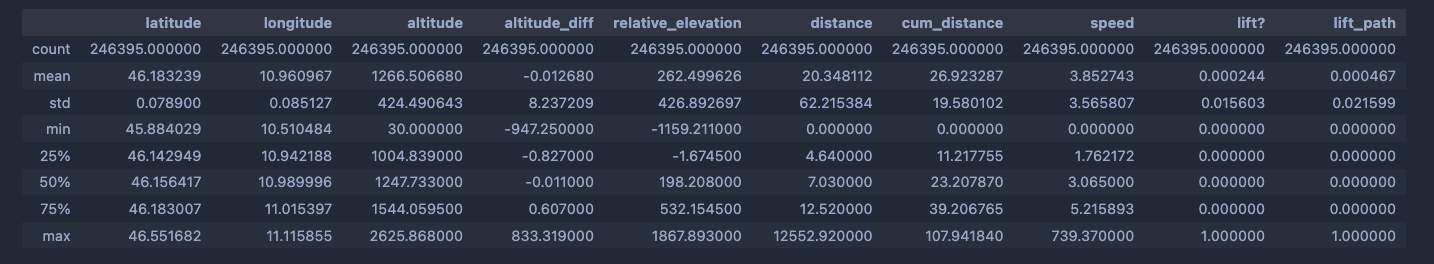
\includegraphics[width=\textwidth]{resources/df_describe.png}
	\caption{The details of all the DataFrames concated together}
	\label{fig:df_describe}
\end{figure}

It can be seen in Fig. \ref{fig:df_describe} that there are 11 columns 
and 246,395 rows in the \texttt{combined\_data}.
Again, the dependent variables and independent variable are extracted from the DataFrame.
To avoid unnecessary duplication, the code for this part is not repeated, as it closely resembles the mentioned codes above.

According to the Fig. \ref{fig:ols}, 
having a lower p-value than alpha, as a result,
all the dependent variables are significant.
\begin{figure}[htb]
	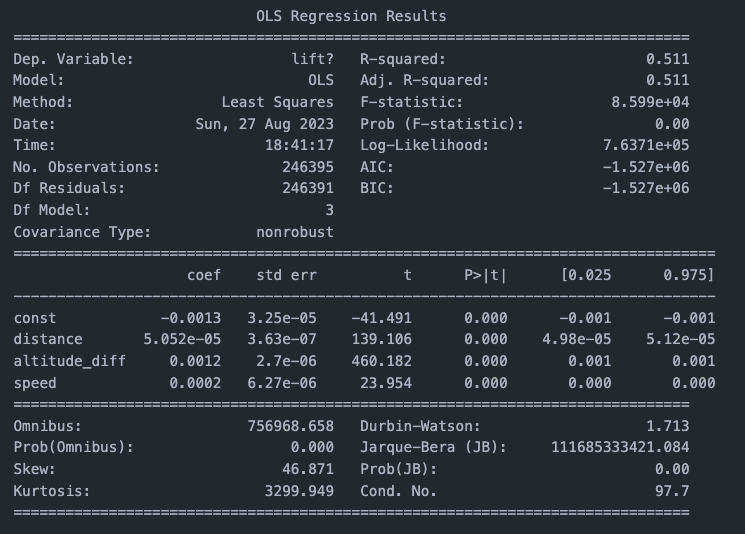
\includegraphics[width=\textwidth]{resources/ols.png}
	\caption{OLS Regression Results on the DataFrames}
	\label{fig:ols}
\end{figure}

\section{Approaches used}

As the project is classification \cite{osisanwo2017supervised}, the following approaches are used.

\subsection{Logistic Regression}
Logistic regression is a common statistical technique adapted for machine learning. It is suited for binary classification tasks where the target variable has two possible classes. Logistic regression models the probability of an observation belonging to each class. The logistic function ensures the probabilities are between 0 and 1 \cite{hosmer2013applied}.

Regression coefficients are learned during training to associate each feature with the log odds of the target. Important considerations when training logistic regressions include handling class imbalance and avoiding overfitting. Regularization methods like L1 and L2 can help prevent overfitting. Logistic regression is easy to implement, fast to train, and interpretable, but may not achieve best-in-class accuracy.


\begin{lstlisting}[language=Python]
from sklearn.linear_model import LogisticRegression


model_lr = linear_model.LogisticRegression(
multi_class="multinomial", solver="lbfgs", max_iter=120, verbose=True)
model_lr.fit(X_train, y_train)
	
\end{lstlisting}


\subsection{Random Forest}

Random forest is an ensemble method that trains multiple decision trees on subsets of data and features, combining their predictions through voting or averaging. By training on subsets, the decision trees exhibit greater diversity, reducing overfitting. Random forests achieve strong predictive accuracy by aggregating across many decision trees to smooth out individual errors \cite{breiman2001random}.

Tuning key hyperparameters like number of trees, maximum depth, and minimum samples per leaf can improve random forest performance. Feature importance scores can be calculated to understand impact on predictions. Random forests are accurate and robust to noise, but lose interpretability compared to simpler models. They can be prone to overfitting with noisy or complex data.



\begin{lstlisting}[language=Python]
from sklearn.ensemble import RandomForestClassifier
from sklearn.metrics import accuracy_score


# Initialize and train the Random Forest model
model_rf = RandomForestClassifier(n_estimators=100, random_state=42)
model_rf.fit(X_train, y_train)

# Make predictions on the testing set
y_pred = model_rf.predict(X_test)

# Evaluate the model"s performance
accuracy = accuracy_score(y_test, y_pred)
print("Accuracy:", accuracy)
\end{lstlisting}



\subsection{Cross validation}
\begin{lstlisting}[language=Python]
from sklearn.model_selection import cross_val_score

# Create a Random Forest classifier
model_rf = RandomForestClassifier(n_estimators=100, random_state=42)

# Perform cross-validation with 5 folds
cross_val_scores = cross_val_score(model_rf, X, y, cv=5, scoring="accuracy")

# Print the cross-validation scores
print("Cross-validation Scores:", cross_val_scores)
print("Mean Accuracy:", cross_val_scores.mean())

\end{lstlisting}


\subsection{Neural Networks}

Artificial neural networks are computing systems inspired by animal brains. They contain interconnected nodes called neurons arranged in layers. Input features are fed into input neurons, transformed through hidden layers of neurons via weighted connections, and output from output neurons. Neural nets learn by adjusting connection weights during training to minimize prediction error \cite{picton1994neural}.

Deep neural networks contain more hidden layers enabling modeling of complex nonlinear relationships in data. Key considerations include network topology and hyperparameter selection. Neural networks can model complex interactions between features that other models may miss. However, they require substantial data for training and are difficult to interpret compared to other techniques.


\begin{lstlisting}[language=Python]
from sklearn.neural_network import MLPClassifier

# Create neural network model
model_nn = MLPClassifier(hidden_layer_sizes=(
	6,), activation="relu", solver="adam", random_state=1)

# Perform 5-fold cross validation
scores = cross_val_score(model_nn, X, y, cv=5)
print("Cross-validation scores: ", scores)

# Train model on training set
model_nn.fit(X_train, y_train)

# Evaluate model performance on test set
print("Test set score: ", model_nn.score(X_test, y_test))

\end{lstlisting}

\section{Conclusion}
\label{sec:model:conclusion}



This section has provided an overview of key machine learning modeling concepts like features, target variables, and training data. Introductory explanations of three major algorithms - logistic regression, 
random forests, and neural networks - were also presented. 
% These descriptions aim to establish essential foundational knowledge before diving into modeling details and experiments in subsequent chapters.